\section{Results}

\subsection{Held-out cohort and class imbalance}
Seven MIT-BIH records, none used for hyperparameter selection or model fitting, contributed 15{,}573 beats to the final test cohort. The distribution was highly uneven: 12{,}061 beats (77.5\%) were normal (N), 2{,}913 (18.7\%) were ventricular ectopic beats (VEB; V), 383 (2.5\%) were fusion beats (F), 214 (1.4\%) were supraventricular ectopic beats (SVEB; S), and only two belonged to the unknown/unclassifiable category (Q). The two common classes consequently dominate accuracy and weighted-F1, whereas the rare rhythms have little influence on either measure. Across the 38 development records, five-fold accuracy was $0.44\pm0.16$, indicating substantial variation across record partitions.

\begin{table*}[t]
  \centering
  \caption{Evaluation cohorts and held-out class distribution. The development and test partitions are separated at the record level. Class counts are shown for the held-out cohort because these are the observations used for the reported final metrics; development class totals are not inferred from the test artifacts.}
  \label{tab:cohort-distribution}
  \begin{tabular}{lcccccccc}
    \toprule
    Cohort & Records & Total beats & N & S (SVEB) & V (VEB) & F & Q & Role \\
    \midrule
    Development & 38 & --- & --- & --- & --- & --- & --- & Tuning, 5-fold CV, final fitting \\
    Held-out test & 7 & 15{,}573 & 12{,}061 & 214 & 2{,}913 & 383 & 2 & Final evaluation only \\
    \bottomrule
  \end{tabular}
\end{table*}


\subsection{Performance relative to evaluated baselines}
Across the three aggregate measures, the CNN--Conformer produced the strongest profile on the common held-out split: accuracy was 0.60 (95\% confidence interval [CI] 0.59--0.60), macro-F1 was 0.26 (95\% CI 0.26--0.27), and weighted-F1 was 0.68 (95\% CI 0.67--0.68) (Table~\ref{tab:test-metrics}; Figure~\ref{fig:model-comparison}). The attention-only network---the strongest competing neural model by held-out accuracy---reached 0.27, 0.15, and 0.38 on the same measures. The absolute differences were 0.33, 0.11, and 0.30. CNN--LSTM and the feature-engineered comparator reached accuracies of 0.18 and 0.14, respectively. Class-specific AUCs were less consistent with an across-the-board advantage; CNN--LSTM, for example, had a slightly higher VEB AUC.

\begin{table*}[t]
  \centering
  \caption{Aggregate performance on the common record-level test set. Values in brackets are 95\% percentile intervals from 1{,}000 beat-level bootstrap samples.}
  \label{tab:test-metrics}
  \begin{tabular}{lccc}
    \toprule
    Model & Accuracy (95\% CI) & Macro-F1 (95\% CI) & Weighted-F1 (95\% CI) \\
    \midrule
    CNN--Conformer & \textbf{0.597 [0.590, 0.605]} & \textbf{0.263 [0.260, 0.267]} & \textbf{0.677 [0.671, 0.684]} \\
    CNN--attention & 0.269 [0.262, 0.277] & 0.149 [0.145, 0.153] & 0.379 [0.370, 0.387] \\
    CNN--LSTM & 0.179 [0.173, 0.185] & 0.154 [0.149, 0.159] & 0.286 [0.278, 0.295] \\
    CNN-only & 0.136 [0.131, 0.142] & 0.069 [0.066, 0.073] & 0.226 [0.218, 0.233] \\
    \bottomrule
  \end{tabular}
\end{table*}


\begin{figure*}[t]
  \centering
  \resizebox{0.94\textwidth}{!}{% AI-assisted data visualization; values are direct transcriptions from qa/claim-ledger.md.
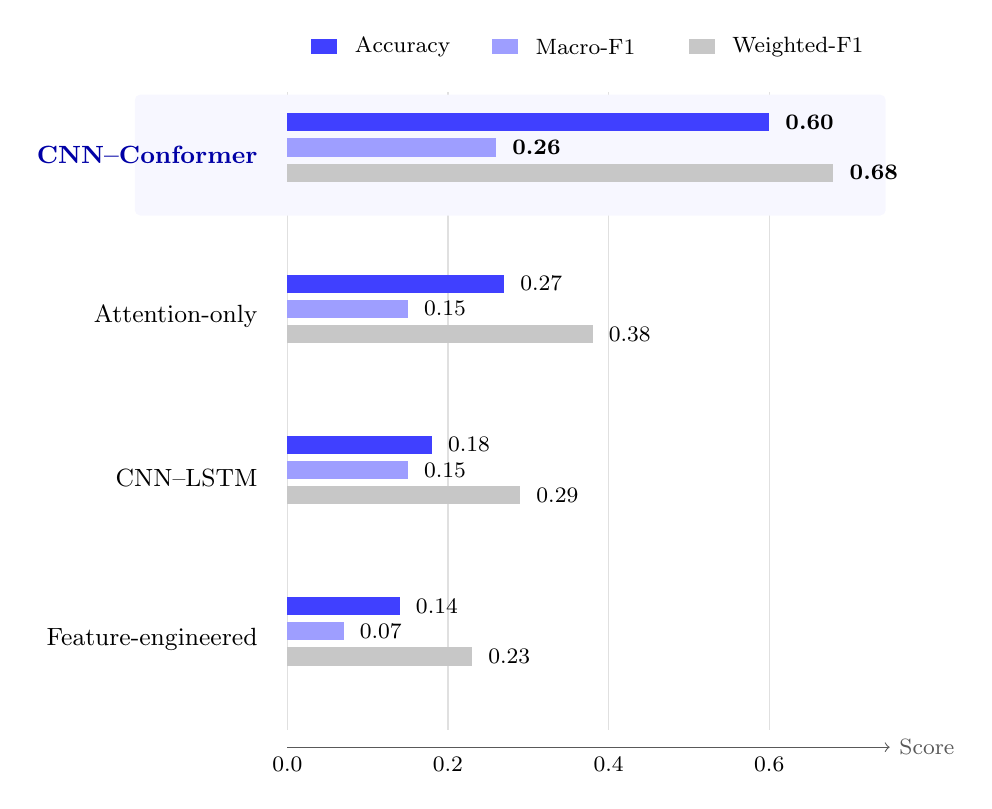
\begin{tikzpicture}[x=10.2cm,y=0.64cm,font=\small]
  % score axis
  \draw[->,black!65] (0,0) -- (0.75,0) node[right,font=\footnotesize]{Score};
  \foreach \x/\lab in {0/0.0,0.2/0.2,0.4/0.4,0.6/0.6} {
    \draw[black!12] (\x,0.35) -- (\x,13.0);
    \node[below,font=\footnotesize] at (\x,0) {\lab};
  }

  % compact legend
  \fill[blue!75] (0.03,13.75) rectangle +(0.032,0.30);
  \node[anchor=west,font=\footnotesize] at (0.072,13.90) {Accuracy};
  \fill[blue!38] (0.255,13.75) rectangle +(0.032,0.30);
  \node[anchor=west,font=\footnotesize] at (0.297,13.90) {Macro-F1};
  \fill[black!22] (0.50,13.75) rectangle +(0.032,0.30);
  \node[anchor=west,font=\footnotesize] at (0.542,13.90) {Weighted-F1};

  % proposed row highlight
  \fill[blue!3,rounded corners=2pt] (-0.19,10.55) rectangle (0.745,12.95);
  \node[anchor=east,font=\small\bfseries,text=blue!65!black] at (-0.025,11.75) {CNN--Conformer};
  \fill[blue!75] (0,12.22) rectangle (0.60,12.58);
  \fill[blue!38] (0,11.72) rectangle (0.26,12.08);
  \fill[black!22] (0,11.22) rectangle (0.68,11.58);
  \node[anchor=west,font=\footnotesize\bfseries] at (0.608,12.40) {0.60};
  \node[anchor=west,font=\footnotesize\bfseries] at (0.268,11.90) {0.26};
  \node[anchor=west,font=\footnotesize\bfseries] at (0.688,11.40) {0.68};

  \node[anchor=east,font=\small] at (-0.025,8.55) {Attention-only};
  \fill[blue!75] (0,9.02) rectangle (0.27,9.38);
  \fill[blue!38] (0,8.52) rectangle (0.15,8.88);
  \fill[black!22] (0,8.02) rectangle (0.38,8.38);
  \node[anchor=west,font=\footnotesize] at (0.278,9.20) {0.27};
  \node[anchor=west,font=\footnotesize] at (0.158,8.70) {0.15};
  \node[anchor=west,font=\footnotesize] at (0.388,8.20) {0.38};

  \node[anchor=east,font=\small] at (-0.025,5.35) {CNN--LSTM};
  \fill[blue!75] (0,5.82) rectangle (0.18,6.18);
  \fill[blue!38] (0,5.32) rectangle (0.15,5.68);
  \fill[black!22] (0,4.82) rectangle (0.29,5.18);
  \node[anchor=west,font=\footnotesize] at (0.188,6.00) {0.18};
  \node[anchor=west,font=\footnotesize] at (0.158,5.50) {0.15};
  \node[anchor=west,font=\footnotesize] at (0.298,5.00) {0.29};

  \node[anchor=east,font=\small] at (-0.025,2.15) {Feature-engineered};
  \fill[blue!75] (0,2.62) rectangle (0.14,2.98);
  \fill[blue!38] (0,2.12) rectangle (0.07,2.48);
  \fill[black!22] (0,1.62) rectangle (0.23,1.98);
  \node[anchor=west,font=\footnotesize] at (0.148,2.80) {0.14};
  \node[anchor=west,font=\footnotesize] at (0.078,2.30) {0.07};
  \node[anchor=west,font=\footnotesize] at (0.238,1.80) {0.23};
\end{tikzpicture}
}
  \caption{Across the common held-out split, the CNN--Conformer has the strongest aggregate profile for accuracy, macro-F1, and weighted-F1 among the evaluated models. Exact values are printed on the bars. TikZ layout was AI-assisted; plotted values are transcribed from archived study metrics.}
  \label{fig:model-comparison}
\end{figure*}

\subsection{Class-specific discrimination and error structure}
Normal and VEB were the only classes with meaningful realised F1. Normal beats had precision 0.95, recall 0.60, and F1 0.74; VEB reached precision 0.48, recall 0.70, and F1 0.57. Their one-vs-rest AUCs were 0.90 (95\% CI 0.89--0.91) and 0.84 (95\% CI 0.84--0.85), respectively. SVEB had F1 0.00 despite an AUC of 0.67, while fusion beats had F1 0.01 with AUC 0.31 (95\% CI 0.29--0.34). With only two test beats, the Q category is included for completeness and does not support substantive class-level interpretation (Table~\ref{tab:class-metrics}; Figure~\ref{fig:class-performance}).

\begin{table*}[t]
  \centering
  \caption{Class-specific performance of the proposed CNN--Conformer on the held-out cohort. The contrast between Normal/VEB and the rare SVEB/Fusion classes is the principal limitation hidden by aggregate metrics. The Q category contains only two beats and is included for completeness rather than substantive inference.}
  \label{tab:class-metrics}
  \begin{tabular}{lrrrrr}
    \toprule
    AAMI class & Support & Precision & Recall & F1 & AUC (95\% CI) \\
    \midrule
    Normal (N) & 12{,}061 & 0.95 & 0.60 & 0.74 & 0.90 [0.89, 0.91] \\
    SVEB (S) & 214 & 0.00 & 0.00 & 0.00 & 0.67 [0.65, 0.68] \\
    VEB (V) & 2{,}913 & 0.48 & 0.70 & 0.57 & 0.84 [0.84, 0.85] \\
    Fusion (F) & 383 & 0.01 & 0.01 & 0.01 & 0.31 [0.29, 0.34] \\
    Unknown (Q) & 2 & 0.00 & 0.00 & 0.00 & 0.59 [0.46, 0.71] \\
    \bottomrule
  \end{tabular}
\end{table*}


\begin{figure*}[t]
  \centering
  \resizebox{0.94\textwidth}{!}{% Vector class-specific comparison of F1 and AUC; values sourced from qa/claim-ledger.md
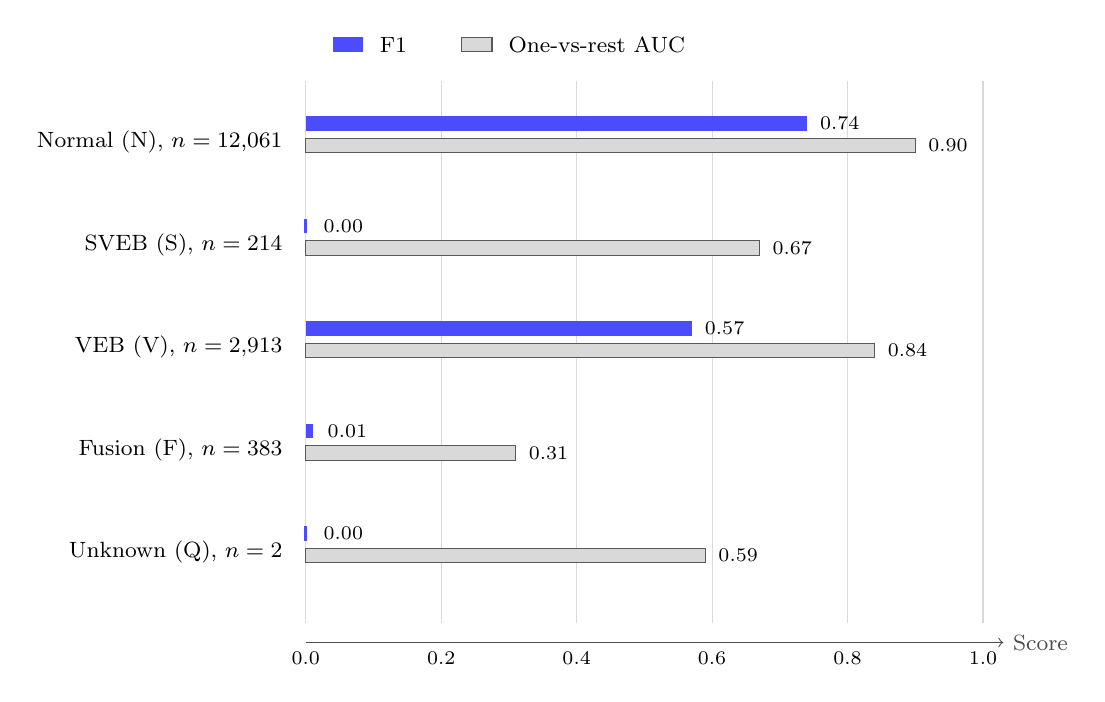
\begin{tikzpicture}[x=8.6cm,y=0.62cm,font=\footnotesize]
  \draw[->,black!70] (0,0) -- (1.03,0) node[right]{Score};
  \foreach \x/\lab in {0/0.0,0.2/0.2,0.4/0.4,0.6/0.6,0.8/0.8,1.0/1.0} {
    \draw[black!15] (\x,0.4) -- (\x,11.5);
    \node[below,font=\scriptsize] at (\x,0) {\lab};
  }
  \fill[blue!70] (0.04,12.1) rectangle +(0.045,0.30);
  \node[anchor=west] at (0.095,12.25) {F1};
  \fill[black!15,draw=black!65] (0.23,12.1) rectangle +(0.045,0.30);
  \node[anchor=west] at (0.285,12.25) {One-vs-rest AUC};
  \node[anchor=east] at (-0.02,10.25) {Normal (N), $n=12{,}061$};
  \fill[blue!70] (0,10.48) rectangle (0.74,10.78);
  \fill[black!15,draw=black!65] (0,10.03) rectangle (0.90,10.33);
  \node[anchor=west,font=\scriptsize] at (0.745,10.63) {0.74};
  \node[anchor=west,font=\scriptsize] at (0.905,10.18) {0.90};
  \node[anchor=east] at (-0.02,8.15) {SVEB (S), $n=214$};
  \draw[blue!70,line width=1.2pt] (0,8.38) -- (0,8.68);
  \fill[black!15,draw=black!65] (0,7.93) rectangle (0.67,8.23);
  \node[anchor=west,font=\scriptsize] at (0.012,8.53) {0.00};
  \node[anchor=west,font=\scriptsize] at (0.675,8.08) {0.67};
  \node[anchor=east] at (-0.02,6.05) {VEB (V), $n=2{,}913$};
  \fill[blue!70] (0,6.28) rectangle (0.57,6.58);
  \fill[black!15,draw=black!65] (0,5.83) rectangle (0.84,6.13);
  \node[anchor=west,font=\scriptsize] at (0.575,6.43) {0.57};
  \node[anchor=west,font=\scriptsize] at (0.845,5.98) {0.84};
  \node[anchor=east] at (-0.02,3.95) {Fusion (F), $n=383$};
  \fill[blue!70] (0,4.18) rectangle (0.01,4.48);
  \fill[black!15,draw=black!65] (0,3.73) rectangle (0.31,4.03);
  \node[anchor=west,font=\scriptsize] at (0.018,4.33) {0.01};
  \node[anchor=west,font=\scriptsize] at (0.315,3.88) {0.31};
  \node[anchor=east] at (-0.02,1.85) {Unknown (Q), $n=2$};
  \draw[blue!70,line width=1.2pt] (0,2.08) -- (0,2.38);
  \fill[black!15,draw=black!65] (0,1.63) rectangle (0.59,1.93);
  \node[anchor=west,font=\scriptsize] at (0.012,2.23) {0.00};
  \node[anchor=west,font=\scriptsize] at (0.595,1.78) {0.59};
\end{tikzpicture}
}
  \caption{Class-level performance is concentrated in Normal and VEB. The SVEB row highlights the central imbalance-related finding: moderate ranking discrimination (AUC 0.67) coexists with realised F1=0.00. Q is visually de-emphasised because only two test beats were available. TikZ layout was AI-assisted; values are transcribed from archived class metrics.}
  \label{fig:class-performance}
\end{figure*}

The minority-class errors were directional rather than diffuse. Of 214 SVEB beats, 151 (71\%) were assigned to Normal and 51 (24\%) to VEB. Among 383 fusion beats, 343 (90\%) were assigned to VEB. The low F1-scores therefore reflect systematic absorption into the more prevalent normal or ventricular categories, not a small number of scattered mistakes (Figure~\ref{fig:error-structure}). The original confusion matrix and one-vs-rest ROC and precision--recall curves are retained as Supplementary Figures~S1--S3.

\begin{figure}[t]
  \centering
  \resizebox{0.98\linewidth}{!}{% AI-assisted explanatory/data figure; values are direct transcriptions from qa/claim-ledger.md.
\begin{tikzpicture}[node distance=0.9cm and 1.45cm,source/.style={rectangle,rounded corners=2pt,draw=blue!65,fill=blue!6,minimum width=2.7cm,minimum height=1.1cm,align=center,font=\footnotesize,thick},target/.style={rectangle,rounded corners=2pt,draw=black!55,fill=black!4,minimum width=2.9cm,minimum height=0.95cm,align=center,font=\footnotesize},note/.style={rectangle,rounded corners=2pt,draw=black!35,fill=black!2,text width=8.8cm,align=left,font=\scriptsize,inner sep=5pt},arrow/.style={-{Stealth[length=4pt]},thick,draw=black!70}]
\node[source] (s) {True SVEB (S)\\$n=214$};
\node[target,right=2.1cm of s,yshift=0.72cm] (sn) {Predicted Normal\\151/214 (71\%)};
\node[target,right=2.1cm of s,yshift=-0.52cm] (sv) {Predicted VEB\\51/214 (24\%)};
\draw[arrow] (s.east) -- (sn.west); \draw[arrow] (s.east) -- (sv.west);
\node[source,below=2.4cm of s] (f) {True Fusion (F)\\$n=383$};
\node[target,right=2.1cm of f] (fv) {Predicted VEB\\343/383 (90\%)};
\draw[arrow] (f.east) -- (fv.west);
\node[note,below=1.25cm of f,anchor=north west] (threshold) at (s.west |- f.south) {\textbf{Post-hoc threshold sweep:} SVEB maximum F1 = 0.06 at threshold 0.09 (precision 0.03, recall 0.90); Fusion maximum F1 = 0.05 at threshold 0.00 (precision 0.02, recall 1.00). Raising minority-class recall therefore produced a large false-positive burden rather than a balanced operating point.};
\end{tikzpicture}
}
  \caption{The dominant rare-rhythm errors are directional: SVEB is largely absorbed into Normal or VEB, and Fusion into VEB. Post-hoc threshold changes increased recall only with very low precision, so a simple operating-point shift did not recover balanced minority-class performance. TikZ layout was AI-assisted; counts and threshold values are transcribed from archived outputs.}
  \label{fig:error-structure}
\end{figure}

\subsection{Post-hoc threshold and calibration analyses}
We used the threshold sweeps to check whether the poor minority-class decisions mainly reflected an unsuitable default operating point. For SVEB, the maximum observed one-vs-rest F1 was 0.06 at a threshold of 0.09, with precision 0.03 and recall 0.90. For fusion beats, the maximum F1 was 0.05 at a threshold of 0.00, with precision 0.02 and recall 1.00. Recall rose only with a very large false-positive burden. Because these sweeps used the stored held-out predictions, they are descriptive and do not constitute independent operating-point selection.

Confidence behaviour was also heterogeneous. Before temperature scaling, the 15-bin expected calibration error (ECE) was 0.417 for normal beats and 0.089 for VEB, with Brier scores of 0.289 and 0.121, respectively. The fitted global temperature ($T=1.050$) changed mean negative log-likelihood only marginally, from 1.047989 to 1.047731. Because the temperature parameter was fitted on the held-out test cohort itself, these values describe calibration behaviour within this cohort only and are not evidence of independent calibration generalisability.
